\chapter{Extracción de información}

Utilizando nuestra página web podemos obtener distintas muestras de Córdoba y Buenos Aires. ¿Cómo podemos analizar estas grabaciones correctamente? Un archivo wav, similar al que se genera en cada una de las muestras, posee muchísima información. Es por esto que debemos seleccionar correctamente qué partes de la información nos sirven y qué partes podemos descartar.

\section{Alineación forzada}

Una grabación a partir de una frase posee muchísima información. Debemos seleccionar qué parte de esta grabación nos interesa y qué parte puede ser descartada. Para ello etiquetamos en qué partes del audio se pronunció cada fonema y también, uniendo cada uno de estos fonemas, etiquetamos cada palabra. Por ejemplo: si tenemos la grabación de la frase \textit{`El canapé salió espectacular’}, utilizamos un archivo aparte que nos dice \textit{`<<espectacular>> se escucha entre el segundo 0.90 y 1.18’}. Lo mismo sucede para cada palabra y fonema de la grabación. Para marcar estas anotaciones utilizamos el formato de archivos TextGrid del programa Praat  \cite{praat}.

Un dato muy importante es que este etiquetado no debe tener que ser realizado con intervención de un humano. Si fuera el caso, tendríamos que hacerlo uno por uno, y al tener muchos audios sería un trabajo muy arduo. De esto se encarga la alineación forzada. Las partes que debemos extraer de los audios son donde se encuentran la diferencias de cada regla descripta anteriormente. 

\subsection{Prosodylab Aligner}

%If you use this tool, we would appreciate it if you cite the following paper:
%Gorman, Kyle, Jonathan Howell & Michael Wagner (2011). Prosodylab-Aligner: A tool for forced alignment of laboratory speech. Proceedings of Acoustics Week in Canada, Quebec City.

Debemos tener una herramienta que nos permita obtener estos pequeños fragmentos de audio para analizar sus diferencias. Usamos una, llamada ProsodyLab Aligner \cite{prosodylab}. Su función es realizar alineaciones automáticas en cada uno de los audios de forma fácil. Analiza uno por uno cada audio y mediante un diccionario determina en qué momento se dijo cada fonema y palabra. 

%parrafo agregado de correcciones de Luciana
Esta actividad se la conoce como alineación forzada. Básicamente consiste en marcar el tiempo desde que comienza y hasta que termina de cada fonema, para todas las grabaciones. Esta se realiza de la siguiente forma: para cada grabación se agrega un archivo que enumera los fonemas que se escuchan en ella. La herramienta analiza las grabaciones y observa cada uno de los fonemas. Si un mismo fonema se utiliza en dos grabaciones, quiere decir que tiene haber características similares en la grabación en ese lapso de tiempo. Utilizando esta idea va prediciendo el lugar de cada fonema. Esta alineación no es perfecta, se puede equivocar en determinar dónde se escucha un fonema, pero es un buen comienzo.  

Una particularidad que se destaca de esta herramienta es que no necesita datos de entrenamiento. Sólo con una hora de grabación es suficiente para correrlo y obtener resultados. Otra característica es que puede utilizarse para cualquier idioma. Esta herramienta está hecha en lenguaje Python (versión 2.5) y sirve como $wrapper$ para utilizar HTK fácilmente. HTK es una biblioteca para crear y manipular Modelos Ocultos de Markov (ver sección \ref{sec:hmm}) fácilmente, y SoX, que nos permite trabajar con audio a través de la consola. 

Los requisitos para utilizar ProsodyLab Aligner son: una hora de grabación con sus transcripciones fonéticas (no necesariamente alineadas a nivel fonético) y un diccionario fonético que nos provea para cada palabra los distintos fonemas que la componen. La hora de grabación la debíamos cumplir recolectando grabaciones de la página web. Esta meta era posible de realizar. La creación de un diccionario fonético era más complicada, ya que debía ser en español. Gracias al \textit{Laboratorio de Investigaciones Sensoriales} \footnote{Este laboratorio depende de CONICET y UBA - Página web: http://www.lis.secyt.gov.ar/} que nos prestó un diccionario, implementado por ellos, pudimos utilizar esta herramienta. Un diccionario fonético es básicamente un listado con las palabras que utilizamos y su transcripción en fonemas. Es importante esto ya que va a ser usado por el alineador para describir los fonemas de cada palabra en cada frase.

%explicación teórica con ejemplo
\subsection{Modelos Ocultos de Markov}
\label{sec:hmm}
Los Modelos Ocultos de Markov \cite{rabiner} (en inglés Hidden Markov Model) son modelos estadísticos por los cuales tratan de predecir estados ocultos a partir de observaciones. Se llaman ``ocultos'' ya que el estado a predecir no se puede observar directamente. Sólo se puede predecir en qué estado oculto está el modelo a través de observaciones. 

Un ejemplo de este modelo podría ser predecir la presión atmosférica observando sólo si el tiempo está lluvioso o seco. Los estados ocultos serían ``Baja'' o ``Alta'' presión atmosférica, que corresponde a lo que queremos saber. Las observaciones para predecir estos estados serían ``Lluvia'' o ``Seco''. En la Figura \ref{ex_hmm} se puede apreciar este ejemplo. Para computar la secuencia más probable de estados ocultos dada una secuencia de observaciones, se utiliza el algoritmo de Viterbi.

\begin{figure}[htbp]
	\begin{center}
		\begin{tikzpicture}[]
		% states
		\node[state] (s1) at (-0.5,2.5) {$Baja$}
		edge [loop above] node[auto,swap,left=2] {$0.3$} ();
		\node[state] (s2) at (2.5,2.5) {$Alta$}
		edge [<-,bend right=40] node[auto,swap] {$0.7$} (s1)
		edge [->,bend left=40] node[auto,swap] {$0.2$} (s1)
		edge [loop above] node[auto,swap,right=2] {$0.8$} ();
		% observations
		\node[observation] (y1) at (-1,0) {$Lluvia$}
		edge [lightedge] node[auto,swap] {$0.6$} (s1)
		edge [lightedge] node[auto,swap] {$0.4$} (s2);
		\node[observation] (y2) at (3,0) {$Seco$}
		edge [lightedge] node[auto,swap] {$0.4$} (s1)
		edge [lightedge] node[auto,swap] {$0.6$} (s2);
		\end{tikzpicture}
	\end{center}
	\caption{Ejemplo de HMM}
	\label{ex_hmm}
\end{figure}

%ejemplo de audio sobre el trabajo
Llevado esta idea a nuestro trabajo, los Modelos Ocultos de Markov tratan de predecir qué fonemas aparecen en cada parte de los audios utilizando la lista de fonemas pronunciada en cada grabación. Mediante este modelo matemático, el programa analiza en cuáles grabaciones, de la misma frase, se produce un mismo patrón de sonido. Si sucede esto en todas estas grabaciones, se lo marca como un fonema de la frase. Ese fonema va a ser marcado de igual forma en el TextGrid de cada una de las grabaciones. Los estados ocultos a predecir son los fonemas de cada frase, en cambio las observaciones provienen del análisis de cada audio. Entonces, a través de muestras va prediciendo los fonemas de las grabaciones.

A continuación se presenta un ejemplo de cómo funcionan estos modelos en nuestro trabajo. 
%
\begin{figure}[h]
	\centering
	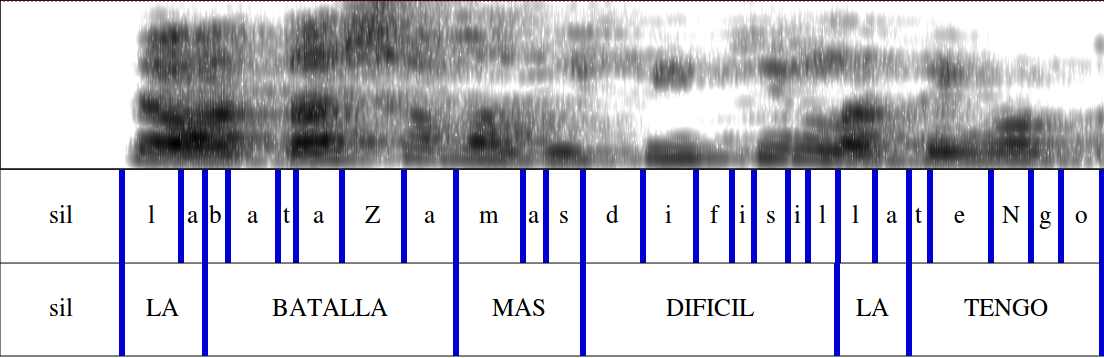
\includegraphics[width=0.8\textwidth]{espectrograma_u3_t33_a1_ver1} \\
	\smallskip
	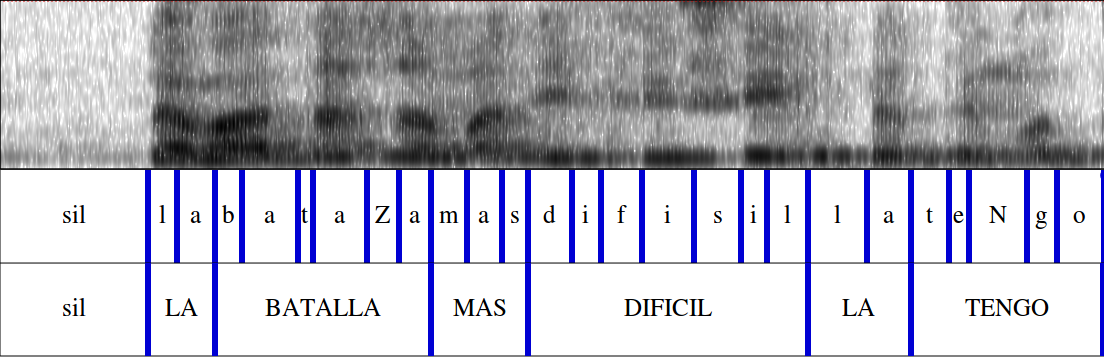
\includegraphics[width=0.8\textwidth]{espectrograma_u27_t33_a1_ver1} 
	\caption{Espectrograma y transcripciones fonética y ortográfica de dos grabaciones producidas por hablantes distintos.}
	\label{car_a1}
\end{figure}
%
La figura \ref{car_a1} muestra las características de grabaciones de la misma frase producidas por dos hablantes distintos. Cada imagen tiene tres capas: el espectrograma de la grabación, su transcripción fonética (comienzo y fin de cada fonema en la grabación) y su transcripción ortográfica (comienzo y fin de cada palabra en la grabación).

Podemos observar que el espectrograma de ambas grabaciones es muy distinto. Si comparamos el mismo fonema en ambos espectrogramas, vemos que son muy diferentes. Aún así la alineación de los fonemas es similar. Si bien no son zonas iguales, poseen similares valores de atributos acústicos para esa región.\footnote{Los atributos acústicos que se emplean son los MFCC, Mel Frequency Cepstral Coefficients, que serán descriptos más adelante, en la sección \ref{sec:atributosacusticos}.} Los Modelos Ocultos de Markov analizan los atributos acústicos y teniendo en cuenta la secuencia de fonemas de la frase, que es idéntica para ambas grabaciones, puede predecir los tiempos de inicio y fin de cada fonema.

%TODO: arreglar sin poner SCORES
%Una vez terminada la alineación, ProsodyLab Aligner genera un archivo donde muestra cómo fueron esas alineaciones utilizando un puntaje. Este archivo se llama \textit{`.SCORES’} y en él se encuentra una lista de todos los audios seguidos de un valor, corresponde a la verosimilitud de las alineaciones. Si una alineación fue similar a otra va a tener aproximadamente un valor similar. En cambio, si posee una alineación muy distinta va a tener valores muy distintos. Este puede ser el primer filtro para el extractor. 
%(TODO CORRECIÓN: PERO QUE ES ESA VEROSIMILITUD)

%Ordenando los audios utilizando esta numeración notamos que los menores poseen alineaciones malas, entonces definimos un umbral arbitrario para el cual aceptar la alineación si este se supera. Si bien este procedimiento es efectivo, notamos que se encuentran algunos falsos positivos, o sea archivos que tienen un buen punto de score pero la alineación es mala. Al tener pocas grabaciones no pudimos aceptar estos casos, debimos corregirlos uno por uno.

\section{Extracción de atributos}

La extracción de atributos fue realizada utilizando el lenguaje Python, que elegimos ya que es fácil de programar y tiene muchas bibliotecas útiles para este tipo de casos. Utilizamos una biblioteca muy conocida llamada Numpy (versión 1.6.1). Esta se utiliza para realizar cálculos matemáticos. Nosotros la utilizamos para tener buena precisión en el cálculo de los atributos.

Después de la alineación realizada, se ejecuta el extractor de atributos. Este posee como input los archivos Wav y TextGrid que corresponden a las alineaciones temporales de cada fonema en cada audio. El diagrama de flujo del extractor se puede ver en la Figura \ref{workflow}. 

La rutina principal del programa toma una por una las grabaciones y su etiquetado asociado. Esta se representa en el componente ``Extractor''. Este llama a distintos componentes que van a calcular cada atributo. Para calcular estos atributos vamos a dividir en dos componentes: ``Extractor temporal'' que se encarga de extraer \textit{atributos temporales} y ``Extractor acústico'' que se encarga de extraer \textit{atributos acústicos}. Los atributos temporales son calculados solamente utilizando el TextGrid, mientras que los atributos acústicos son calculados usando tanto el TextGrid como el archivo de audio. Si el atributo está presente en la grabación, tendremos ese dato en la extracción; si no, se dejará como desconocido. Luego de calculado todos sus atributos para cada grabación, juntamos todos los resultados y generamos el archivo Arff utilizando el componente ``Generador de archivo Arff''.

En el archivo Arff cada línea representa una grabación.  Cada una de estas lineas posee todos los resultados del cálculo de los atributos separado por comas. Cada uno de estos atributos corresponde al cálculo de una regla correspondiente. Necesitamos utilizar este formato ya que es necesario para ingresar datos en Weka, la plataforma que elegimos para correr algoritmos de \textit{machine learning}. Veamos cada uno de los dos tipos de atributos.

\begin{figure}[h!]
    \centerline{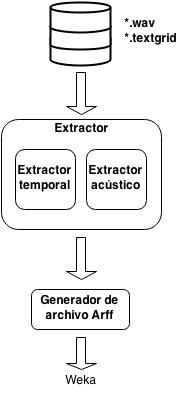
\includegraphics[width=0.2\textwidth]{diagrama_workflow1} }
    \caption{Diagrama de flujo}
    \label{workflow}
\end{figure}

\subsection{Atributos temporales}

Los atributos temporales corresponden a atributos sobre la duración de los fonemas y las sílabas de cada grabación. Para calcularlos utilizamos como input el TextGrid generado en la alineación. Los atributos temporales se dividen en dos grupos: fonéticos y silábicos. 

Básicamente estas funciones recorren el TextGrid buscando un patrón en particular y miden su duración. Se mide la cantidad de ocurrencias que posee y luego se realiza su normalización de dos formas posibles. 

La primera normalización, conocida como z-score, será utilizando la forma:

\hspace{2cm} \[\frac{ X - \mu }{ \sigma }\]

\noindent donde:

\begin{itemize}
	\item $X$ es el valor a normalizar (por ejemplo: la duración de un fonema dado).
	\item $\mu$ es el promedio de duración de la unidad utilizada en la grabación.
	\item $\sigma$ es el desvío estándar de la unidad utilizada en la grabación.
\end{itemize}

\noindent Y luego la segunda suponiendo que $\mu = 0$ (o bien, que la media no afecta negativamente los cómputos posteriores):

\hspace{2cm} \[\frac{ X }{ \sigma }\]

\noindent Esta última tiene el nombre de Half-normal Distribution.

El valor a normalizar puede variar: mientras uno va a tener en cuenta fonemas, el otro tiene en cuenta sílabas. Debemos utilizar los datos normalizados ya que necesitamos atributos que nos muestren, para un hablante en particular, si el fonema en cuestión es relevante con respecto a los demás de la grabación. Al normalizar un atributo vemos cuán fuera de lo común resulta en el marco de \textit{ese} hablante en particular en \textit{esa} grabación. No importa si habla lento o rápido. Lo importante es la relación del fonema a medir con respecto a los demás. Lo mismo sucede para las sílabas. Si utilizáramos valores absolutos, se perdería esta relación ya que variaría con respecto a la velocidad del habla de cada hablante y cada grabación.
 
A continuación veamos los atributos en particular para cada uno de los grupos y cómo se realiza su cálculo. Para la regla 1 vamos a definir atributos silábicos, ya que corresponde a reglas que están definidas para sílabas, mientras que para las demás reglas (2 al 6) vamos a definir atributos fonéticos.

\subsubsection{Atributos fonéticos}

Los atributos que contabilizan fonemas son:

\begin{itemize}
    \item \textbf{Duración de `kt’:} en este atributo buscamos el patrón /kt/ en los TextGrids y luego, en ese intervalo, medimos la duración del fonema /k/. Este atributo intenta extraer la diferencia explicada en la regla 4, que nos indica la duración de dicho fonema.
    \item \textbf{Duración de `sc’:} ídem con /sc/ y midiendo el fonema /s/. Este corresponde a la regla 3 que referencia a la duración del fonema /s/ anterior a /c/.  
    \item \textbf{Duración de la `ll’:} buscamos el patrón /ll/ y medimos su duración. Este atributo hace referencia a la regla 5 que mide dicho fonema.
    \item \textbf{Duración de `rr’:} ídem para /r/ fuerte. Referencia a la regla 6 que hace hincapié en este fonema.
    \item \textbf{Duración de `s’ final:} ídem para las /s/ de final de palabra. Corresponde a la regla 2 que hace referencia a la aspiración de la /s/ de final de las palabras.  
    \item \textbf{Duración de todos los fonemas:} este atributo suma la duración y la cantidad de todos los fonemas de una grabación y luego realiza su promedio. En este caso no se realiza normalización, ya que no se está tratando de analizar si un fonema en particular es destacado en comparación con los demás, sino que se trata de ver la duración en promedio de todos los fonemas en una grabación.
    \item \textbf{Duración de todas las vocales:} medimos la duración media de todas las vocales (juntas). Luego normalizamos para conocer la relación entre la duración de las vocales respecto de la duración de todos los fonemas.
    \item \textbf{Duración de todas las consonantes:} ídem anterior para todas las consonantes (juntas). 
\end{itemize}

El cálculo de un atributo fonético se realiza de la siguiente manera: supongamos por ejemplo que queremos calcular la duración de `kt’ en la frase \textbf{\textit{``En la pelea se conoce al soldado solo en la victoria se conoce al caballero’’}}. Analizamos el TextGrid asociado a la grabación que nos proveerá en qué instante se produjo cada fonema. Los fonemas en esta frase van a ser \textbf{\textit{``en la pelea se konose al soldaDo solo en la biktorja se konose al kaBaZero’’}}. En la Figura \ref{ejemploAtribFon} se puede ver una representación gráfica del TextGrid marcando los tiempos para cada fonema\footnote{Aclaración: la duración de los fonemas varia muchísimo. En el ejemplo se simplificó marcando todos los tiempos con el mismo tamaño para hacer más simple la figura.}. Se marca en negro el segmento donde aparece la `k’.

Los valores de la normalización serán: para $\mu$ se calculará como el promedio de duración de los fonemas en la frase en cuestión. Viendo la Figura \ref{ejemploAtribFon} será el promedio de los tiempos marcados para todos los fonemas. $\sigma$ será el desvío estándar de la duración de todos los fonemas de la frase. Y $X$ será el promedio de duración de los fonemas de la forma /k/ en el intervalo /kt/ correspondiente. La única aparición de este fonema es en la palabra ``biktorja’’ y en el gráfico está marcado en negro. La misma idea se aplica en el cálculo de los demás atributos.

\begin{figure}[H]
\centering
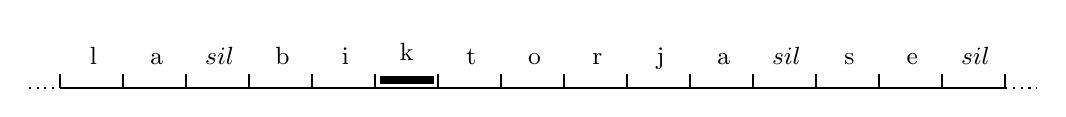
\begin{tikzpicture}[xscale=0.8]
\draw[x=2cm,step=0.05pt,thick,>=latex](0,0) -- (7.5,0);
\foreach \Xc in {0,...,15}
{
	\draw[thick] 
	(\Xc,0) -- ++(0,05pt);
}
\draw[dotted,thick] (-0.5,0) -- (0,0);
\draw[dotted,thick] (15,0) -- (15.5,0);
% la victoria se conoce
\foreach \Xc/\Texto in 
{5/k}
{
	\fill[black] 
		([xshift=2pt]\Xc,0.05)  
			rectangle node[above] {\strut\small\Texto} 
		([xshift=-2pt]\Xc+1,0.15);  
}
\foreach \Xc/\Texto in 
{0/l,1/a,2/$sil$,3/b,4/i,6/t,7/o,8/r,9/j,10/a,11/$sil$,12/s, 13/e, 14/$sil$}
{
	\node[above] at ([xshift=15pt]\Xc,0.05){\strut\small\Texto} ;
}
\end{tikzpicture}
\caption{Ejemplo de cálculo de atributo}
\label{ejemploAtribFon}
\end{figure}

En definitiva, se busca el patrón definido por el atributo, se mide la cantidad de ocurrencias que posee y luego se realiza su normalización de las dos formas utilizando esos valores. 

\subsubsection{Atributos silábicos}

Los atributos que contabilizan sílabas usados son:

\begin{itemize}
    \item \textbf{Duración de la sílaba acentuada:} en cada una de las grabaciones buscamos la sílaba acentuada de cada palabra, medimos su duración y normalizamos con las demás sílabas de la frase. Ésto lo realizamos recorriendo su TextGrid asociado.
    \item \textbf{Duración de la sílaba anterior a la acentuada:} realizamos el mismo calculo anterior pero con la sílaba previa a la acentuada. 
\end{itemize}

Veamos cómo se realiza el cálculo de un atributo silábico: supongamos que queremos calcular el atributo que corresponde a la duración de la sílaba anterior a la acentuada y lo realizamos para la misma frase que en el caso anterior. $\mu$ representará el promedio de duración de las sílabas en la frase. $\sigma$ será el desvío estándar de la duración de estas sílabas en la frase. Y finalmente $X$ será el promedio de duración de las sílabas anteriores a las acentuadas. Para cada uno de estos valores se calculan los dos tipos de normalización. En la Figura \ref{ejemploAtribSil} podemos ver este ejemplo gráficamente\footnote{Aclaración: al igual al caso anterior, la duración de las sílabas varia muchísimo. En el ejemplo se simplificó marcando todos los tiempos con el mismo tamaño para ser más simple la figura.}. No pudimos escribir toda la frase y todos sus acentos por cuestiones de espacio. 

En la frase del ejemplo marcamos las sílabas anteriores a la acentuada para distinguirlas. El analizador, cuando calcule este atributo, va a identificar las sílabas acentuadas y tomará su antecesora. 

\begin{figure}[H]
	\centering
	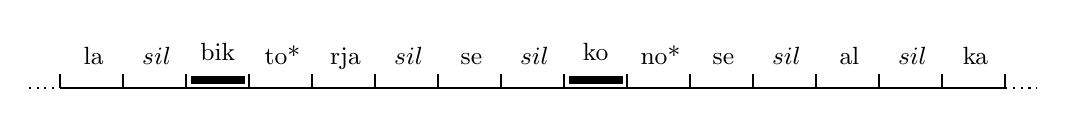
\begin{tikzpicture}[xscale=0.8]
	\draw[x=2cm,step=0.05cm,thick,>=latex](0,0) -- (7.5,0);
	\foreach \Xc in {0,...,15}
	{
		\draw[thick] 
		(\Xc,0) -- ++(0,05pt);
	}
	\draw[dotted,thick] (-0.5,0) -- (0,0);
	\draw[dotted,thick] (15,0) -- (15.5,0);
	% la victoria se conoce
	\foreach \Xc/\Texto in 
	{2/bik,8/ko}
	{
		\fill[black] 
		([xshift=2pt]\Xc,0.05)  
		rectangle node[above] {\strut\small\Texto} 
		([xshift=-2pt]\Xc+1,0.15);  
	}
	\foreach \Xc/\Texto in 
	{0/la,1/$sil$,3/to*,4/rja,5/$sil$,6/se,7/$sil$,9/no*,10/se,11/$sil$,12/al, 13/$sil$, 14/ka}
	{
		\node[above] at ([xshift=15pt]\Xc,0.05){\strut\small\Texto} ;
	}
	\end{tikzpicture}
	\caption{Ejemplo de cálculo de atributo}
	\label{ejemploAtribSil}
\end{figure}

 Para saber cuál es la sílaba acentuada se realizó una tabla que describe para cada frase cuáles son sus sílabas acentuadas. Este se encuentra en el apéndice de este informe. Estos atributos los usamos para poder medir la regla 1, la más prominente de la tonada cordobesa.

\subsection{Atributos acústicos}
\label{sec:atributosacusticos}
Los atributos acústicos utilizan las propiedades de las grabaciones realizadas. Para ello debimos extraer información con algún método que permita medirlos. Elegimos el calculo de coeficientes cepstrales en escala de mel (en inglés MFCC: Mel Frequency Cepstral Coefficient) ya que tiene relación directa con la percepción auditiva humana. Veamos el cálculo de estos coeficientes.

La forma en que hablamos se produce por el movimiento de varias articulaciones en nuestra boca. Estas conectan a dientes, lengua, tráquea, etc. Estas articulaciones trabajan en conjunto para darle forma al sonido producido. 

El tracto vocal suele modificarse de manera bastante lenta y se la puede considerar constante en intervalos de alrededor de 10 a 20 ms. Por otro lado, la señal de audio poseen muchas variaciones continuamente. Para minimizar las discontinuidades de la señal se aplica un ventaneo sobre la señal del habla. 

Las ventanas consecutivas, aplicadas a la señal del habla, se solapan. Esto permite evitar las transiciones abruptas de la señal. Las ventanas empleadas son de 20 a 40 ms de duración, pero los vectores de atributos suelen calcularse cada 10 ms. Estos intervalos son conocidos como trama o frame. Este ventaneo se puede apreciar en la Figura \ref{ej_mfcc_graf}.

\newcommand{\mfccvec}[3]% x, y
{  
	\node[fill={rgb:black,1;white,2;white,3}, rounded corners, draw, inner sep=+0pt] at (#1,#2) {\tiny \begin{tabular}{c}
		Coef 1\\\hline
		Coef 2\\\hline
		Coef 3\\\hline
		...\\\hline
		Coef N\\
	\end{tabular}};
	\node at (#1, #2-1) {{\tiny #3}};
}

\newcommand{\mfccvecmax}[3]% x, y
{  
	\node[fill={rgb:red,1;white,2;white,3}, rounded corners, draw, inner sep=+0pt] at (#1,#2) {\tiny \begin{tabular}{c}
		Max(T1.coef1, T2.coef1, ... , TM.coef1)\\\hline
		Max(T1.coef2, T2.coef2, ... , TM.coef2)\\\hline
		Max(T1.coef3, T2.coef3, ... , TM.coef3)\\\hline
		...\\\hline
		Max(T1.coefN, T2.coefN, ... , TM.coefN)\\
	\end{tabular}};
	\node at (#1, #2-1) {{\tiny #3}};
}

\newcommand{\intervalo}[2]% x, y
{  
	\draw (#1,#2) -- (#1+0.8,#2);
	\draw (#1,#2-.1) -- (#1, #2+.1);
	\draw (#1+0.8,#2-.1) -- (#1+0.8, #2+.1);

	\draw (#1,#2) -- (#1+.1,#2+.05);
	\draw (#1,#2) -- (#1+.1,#2-.05);

	\draw (#1+0.8,#2) -- (#1+0.8-.1,#2+.05);
	\draw (#1+0.8,#2) -- (#1+0.8-.1,#2-.05);
}

\begin{figure}[H]
	\begin{center}		
		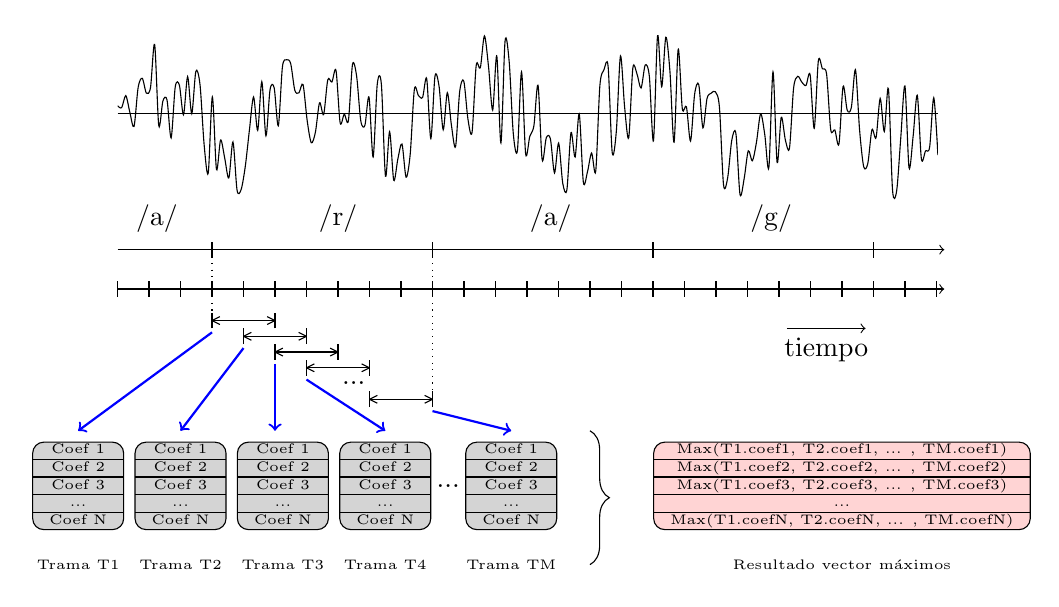
\begin{tikzpicture}[samples=200, domain=0:5*360]
		\begin{axis}[
		width=12cm, height=4cm,
		enlarge x limits=false,
		xtick=\empty,
		axis lines*=middle,
		hide y axis
		]
		\addplot [no markers, smooth] {sin(x)+rand*2};
		\end{axis}
		
		\def \posy {-1};

		%flecha tiempo
		\draw [->] (8.5,-0.5+\posy) -- (9.5,-0.5+\posy);
		\node [align=center,below] at (9,-0.5+\posy) {tiempo};

		%grilla fonetica
		\draw [->] (0,0.5+\posy) -- (10.5,0.5+\posy);
		\draw (1.2,-.1+0.5+\posy) -- (1.2, .1+0.5+\posy);
		\node [align=center,below] at (0.5,1.2+\posy) {/a/};
		\draw (4,-.1+0.5+\posy) -- (4, .1+0.5+\posy);
		\node [align=center,below] at (2.8,1.2+\posy) {/r/};
		\draw (6.8,-.1+0.5+\posy) -- (6.8, .1+0.5+\posy);
		\node [align=center,below] at (5.5,1.2+\posy) {/a/};	
		\draw (9.6,-.1+0.5+\posy) -- (9.6, .1+0.5+\posy);
		\node [align=center,below] at (8.3,1.2+\posy) {/g/};
		
		%linea vertical
		\draw[dotted] (1.2,0.5+\posy) -- (1.2,-0.4+\posy);
		\draw[dotted] (4,0.5+\posy) -- (4,-1.4+\posy);
		
		%grilla
		\draw [->] (0,0+\posy) -- (10.5,0+\posy);	
		\foreach \r in {0,0.4,0.8,...,10.5}
			\draw (\r,-.1+\posy) -- (\r, .1+\posy);

		%ventanas
		\intervalo{1.2}{-0.4+\posy};
		\intervalo{1.6}{-0.6+\posy};
		\intervalo{2}{-0.8+\posy};
		\intervalo{2.4}{-1+\posy};
		\node at (3,-1.2+\posy) {...};
		\intervalo{3.2}{-1.4+\posy};
		
		\mfccvec{-0.5}{-2.5+\posy}{Trama T1};
		\draw[blue, thick,->] (1.2,-0.55+\posy) -- (-0.5,-1.8+\posy);
		
		\mfccvec{0.8}{-2.5+\posy}{Trama T2};
		\draw[blue, thick,->] (1.6,-0.75+\posy) -- (0.8,-1.8+\posy);
		
		\mfccvec{2.1}{-2.5+\posy}{Trama T3};
		\draw[blue, thick,->] (2,-0.95+\posy) -- (2,-1.8+\posy);
		
		\mfccvec{3.4}{-2.5+\posy}{Trama T4};
		\draw[blue, thick,->] (2.4,-1.15+\posy) -- (3.4,-1.8+\posy);
		
		\node at (4.2, -2.5+\posy) {...};
		\mfccvec{5}{-2.5+\posy}{Trama TM};
		\draw[blue, thick,->] (4,-1.55+\posy) -- (5,-1.8+\posy);
		
		%resultado
		\mfccvecmax{9.2}{-2.5+\posy}{Resultado vector máximos}
		\draw[decorate,decoration={brace,amplitude=7pt}] (6,-1.8+\posy) -- (6,-3.5+\posy);

	\end{tikzpicture}
	\end{center}
	\caption{Representación del cálculo de MFCC: al encontrar el fonema /r/ aplicamos el ventaneo en toda su duración. Para cada uno de ellos, se calcula los coeficientes MFCC. Finalmente se arma una traza con los máximos de cada coeficiente. Ídem para el mínimo y promedio.}
	\label{ej_mfcc_graf}
\end{figure}

Luego de tener separada la señal en pequeñas tramas, para cada una de ellas se calcula la Transformada Discreta de Fourier. Posteriormente se utiliza un banco de filtros solapados y espaciados uniformemente sobre la escala de Mel (conocido en inglés como Mel Filterbank). Como dijimos antes, esta escala es importante ya que representa la percepción auditiva humana. A los valores de energía que superaron este filtro se les aplica logaritmo. Para finalizar, a estos se les aplica la Transformada Discreta del Coseno.

%El siguiente pseudocódigo explica paso a paso cómo se calculan los coeficientes:
%\begin{lstlisting}[numbers=none, keywordstyle=\ttfamily]
%   MFCC (Mel frequency cepstral coefficient):
%   1) Partir la señal en pequeñas tramas 
%   2) Para cada frame estimar su espectro de energía utilizando Transformada Rapida de Fourier (FFT)
%   3) Aplicar el banco de filtros solapados sobre escala mel. Sumar los valores en cada filtro
%   4) Aplicar logaritmo a los valores de cada filtro
%   5) Aplicar Transformada de Coseno Discreta
%   6) Los MFCC son las amplitudes del espectro resultante.
%\end{lstlisting}

Terminado el algoritmo obtenemos 13 atributos acústicos de ese segmento. Agregamos también la derivada de estos atributos y la segunda derivada que representan las variaciones temporales. En total derivando dos veces llegan a 39 atributos acústicos. Debemos extraer estas métricas para cada una de las grabaciones.

Este cálculo de vectores de MFCC lo realizamos entre el principio y fin de cada atributo que represente una regla. Por ejemplo como observamos en la Figura \ref{ej_mfcc_graf}: si encontramos el atributo fonético /r/, calculamos los vectores MFCC en el intervalo donde suena este fonema. Con éstos vectores, calculamos el valor máximo, mínimo y promedio para cada enésima posición y armamos tres vectores con estos valores. O sea, el vector de valores máximos tendrá en su primer elemento el valor máximo de los primeros elementos de todos los vectores, así sucesivamente. Ídem para el vector mínimo y promedio. 

Para realizar el cálculo de estos coeficientes se utilizó un script en Matlab\footnote{El creador del script es Kamil Wojcicki y se puede descargar de la página web http://www.mathworks.com/matlabcentral/fileexchange/32849-htk-mfcc-matlab/}. Este calcula  sus primeras y segundas derivadas. El extractor necesita estos valores para cada audio a extraer, es por eso que se conecta con Matlab a través de un wrapper para ejecutar el script y luego continuar con la extracción.

%versión nueva
%Los atributos acústicos utilizan las propiedades de las grabaciones realizadas. Para ello debimos extraer información con algún método que permita medirlos. Elegimos el calculo de MFCC ya que tiene relación directa con la percepción auditiva humana. 
%
%%\subsubsection{Mel Frequency Cepstral Coefficients}
%
%%http://practicalcryptography.com/miscellaneous/machine-learning/guide-mel-frequency-cepstral-coefficients-mfccs/
%
%La forma en que hablamos se produce por varias articulaciones, tales como dientes, lengua, tráquea etc. Estas articulaciones trabajan para darle forma y aplicarle un filtro al sonido producido. Si sabemos correctamente qué filtro se aplica, podremos saber qué sonido producen. La forma y el filtro asociado nos muestran dónde está la fuerza en el fonema. Este filtro es muy importante para entender la percepción humana. Los coeficientes MFCC se encargan de representar estos filtros. Veamos cómo se calculan.
%
%Las señales de audio poseen muchas variaciones continuamente. En períodos cortos de tiempo, estas variaciones se reducen. Supongamos que dividimos cada audio en pequeños frames para calcular en ellos los coeficientes. El tamaño de cada frame está entre 20-40 ms. Si la variación es menor que esta duración la descartamos.
%
%Luego para cada frame se calcula el espectro de frecuencia. Esto viene motivado por un órgano que se encuentra en la oreja llamado Cóclea. Éste vibra de diferente forma al llegarle cada frecuencia del sonido. Al vibrar, activa nervios que representan las distintas frecuencias que escuchamos. Dividir el sonido en períodos intenta mostrar qué frecuencias están activas.
%
%La Cóclea no reconoce diferencias entre dos frecuencias muy cercanas. Esto se incrementa mientras más alta es la frecuencia. Para representar esta idea se utiliza un filtrado por escala de Mel. Esta escala es una aproximación de nuestra percepción. A frecuencias menores a los 1 Khz el filtro se comporta de forma lineal. A partir de ese valor, se comporta de forma logarítmica. 
%
%%http://i.stack.imgur.com/YUH48.gif
%
%% Aca se introduce los filtros onda serrucho. 
%Mientras más aumentamos la frecuencia, más anchos son los filtros aplicados. Por ejemplo, ya en 4 Khz se aplican 20 filtros. Lo importante es ver cuánta energía hay en las frecuencias involucradas en el filtro. Luego que tenemos la energía de estos tramos le aplicamos la función logaritmo. De esta forma, para valores grandes de frecuencias su valor se decrementará y no será igual que las pequeñas que poseen forma lineal. Esto se ajusta mejor a cómo escucha el oído. Para finalizar se computa DCT de las energías filtradas. 
%
%El siguiente pseudocódigo explica paso a paso cómo se calculan los coeficientes:
%\lstset{ %
%language=C++,                % choose the language of the code
%basicstyle=\footnotesize,       % the size of the fonts that are used for the code
%numbers=left,                   % where to put the line-numbers
%numberstyle=\footnotesize,      % the size of the fonts that are used for the line-numbers
%stepnumber=1,                   % the step between two line-numbers. If it is 1 each line will be numbered
%numbersep=5pt,                  % how far the line-numbers are from the code
%backgroundcolor=\color{white},  % choose the background color. You must add \usepackage{color}
%showspaces=false,               % show spaces adding particular underscores
%showstringspaces=false,         % underline spaces within strings
%showtabs=false,                 % show tabs within strings adding particular underscores
%frame=single,           % adds a frame around the code
%tabsize=2,          % sets default tabsize to 2 spaces
%captionpos=b,           % sets the caption-position to bottom
%breaklines=true,        % sets automatic line breaking
%breakatwhitespace=false,    % sets if automatic breaks should only happen at whitespace
%escapeinside={\%*}{*)}          % if you want to add a comment within your code
%}
%\begin{lstlisting}
%  MFCC (Mel frequency cepstral coefficient):
%  1) Aplicar la derivada de Fourier de la se~nal. -> Espectro
%  2) Mapear las amplitudes del espectro a la escala mel.  
%  3) Calcular el logaritmo.
%  4) Aplicar la transformada de coseno discreta (DCT).
%  5) Los MFCC son las amplitudes del espectro resultante.
%\end{lstlisting}
%
%Este algoritmo se calcula para un segmento del audio. Como dijimos, el audio se debe dividir en frames de 20 o 30 milisegundos pero avanzando 10 o 15 milisegundos. Es por ello que hay superposiciones en cada segmento. Al finalizar el algoritmo obtenemos 13 atributos acústicos de ese segmento. Podemos realizar la derivada de estos atributos y la segunda derivada representa las variaciones temporales. En total derivando dos veces llegan a 33 atributos acústicos. Debemos extraer estas métricas para cada uno de los Wavs grabados.
%
%Para realizar el cálculo de estos coeficientes se utilizó un script en Matlab. El creador del script es Kamil Wojcicki y utiliza los 33 atributos utilizando sus primeras y segundas derivadas. El extractor necesita estos valores para cada audio a extraer. Es por eso que se conecta con Matlab a través de un wrapper para ejecutar el script y luego continuar con la extracción.

\subsection{Atributos desconocidos}

Una grabación no puede definir todos los atributos que declaramos. Cada frase define sólo algunos atributos y los demás no sabe cuál es su posible valor. Es por eso que debemos tomar una decisión sobre qué hacer con los atributos que no conocemos. 

Determinamos que a los atributos que no pudieron ser extraídos en la grabación los marcaremos como desconocidos. Si para una grabación un atributo es desconocido, no vamos a poder saber ese valor para ese hablante. Debemos analizar otra grabación del mismo hablante que defina ese atributo.

\subsection{Nomenclatura utilizada}
Para referenciar cada uno de los atributos debimos definir una nomenclatura. La definición que tomamos es la siguiente:
\begin{center}
\textit{TIPO+``\_''+ATRIBUTO+``\_''+NORMALIZACIÓN} 
\end{center}

\begin{itemize}
  \item \emph{TIPO:} puede ser \emph{FON, SIL o ACU}. Esto corresponde al tipo de atributo, si es fonético, silábico o acústico.
  \item \emph{ATRIBUTO:} puede ser \emph{kt, ll, sc, rr, Sfinal, vowel o consonant} haciendo alusión a cada una de los atributos. También aquí se encuentran los atributos generados por MFCC cuyos nombres son de la forma \emph{(Min $|$ Max $|$ Avg) + (KT $|$ LL $|$ SC $|$ RR)}. Para hacer referencia a las reglas sobre atributos silábicos utilizamos los nombres de \emph{syllableAccent} y \emph{prevSyllableAccent} para la duración de la sílaba acentuada y de la sílaba anterior a esta.
  \item \emph{NORMALIZACIÓN:} corresponde al tipo de normalización realizada. Estas pueden ser \emph{norm} haciendo alusión a z-score o \emph{normhd} haciendo alusión a normalización tomando $mu=0$.
\end{itemize}
 
Por ejemplo: definimos \textit{SIL\_prevSyllableAccent\_normhd} como la duración de la silaba anterior a la acentuada aplicando normalización con $mu=0$. Todos los nombres y a qué atributo se refieren se pueden ver en el apéndice de atributos.

En la próxima sección veremos los audios obtenidos en este experimento para luego analizar los atributos de cada uno.